%%%%%%%%%%%%%%%%%%%%%%%%%%%%%%%%%%%%%%%%%%%%%%%%%%%%%%%%%%%%%%%%%%%%%%%%%%%%%%%%%%%%%%%%%%%%%%%%
%
% CS484 Written Question Template
%
% Acknowledgements:
% The original code is written by Prof. James Tompkin (james_tompkin@brown.edu).
% The second version is revised by Prof. Min H. Kim (minhkim@kaist.ac.kr).
%
% This is a LaTeX document. LaTeX is a markup language for producing 
% documents. Your task is to fill out this document, then to compile 
% it into a PDF document. 
%
% 
% TO COMPILE:
% > pdflatex thisfile.tex
%
% If you do not have LaTeX and need a LaTeX distribution:
% - Personal laptops (all common OS): www.latex-project.org/get/
% - We recommend latex compiler miktex (https://miktex.org/) for windows,
%   macTex (http://www.tug.org/mactex/) for macOS users.
%   And TeXstudio(http://www.texstudio.org/) for latex editor.
%   You should install both compiler and editor for editing latex.
%   The another option is Overleaf (https://www.overleaf.com/) which is 
%   an online latex editor.
%
% If you need help with LaTeX, please come to office hours. 
% Or, there is plenty of help online:
% https://en.wikibooks.org/wiki/LaTeX
%
% Good luck!
% Min and the CS484 staff
%
%%%%%%%%%%%%%%%%%%%%%%%%%%%%%%%%%%%%%%%%%%%%%%%%%%%%%%%%%%%%%%%%%%%%%%%%%%%%%%%%%%%%%%%%%%%%%%%%
%
% How to include two graphics on the same line:
% 
% \includegraphics[\width=0.49\linewidth]{yourgraphic1.png}
% \includegraphics[\width=0.49\linewidth]{yourgraphic2.png}
%
% How to include equations:
%
% \begin{equation}
% y = mx+c
% \end{equation}
% 
%%%%%%%%%%%%%%%%%%%%%%%%%%%%%%%%%%%%%%%%%%%%%%%%%%%%%%%%%%%%%%%%%%%%%%%%%%%%%%%%%%%%%%%%%%%%%%%%

\documentclass[11pt]{article}

\usepackage[english]{babel}
\usepackage[utf8]{inputenc}
\usepackage[colorlinks = true,
            linkcolor = blue,
            urlcolor  = blue]{hyperref}
\usepackage[a4paper,margin=1.5in]{geometry}
\usepackage{stackengine,graphicx}
\usepackage{fancyhdr}
\setlength{\headheight}{15pt}
\usepackage{microtype}
\usepackage{times}
\usepackage{booktabs}

% From https://ctan.org/pkg/matlab-prettifier
\usepackage[numbered,framed]{matlab-prettifier}

\frenchspacing
\setlength{\parindent}{0cm} % Default is 15pt.
\setlength{\parskip}{0.3cm plus1mm minus1mm}

\pagestyle{fancy}
\fancyhf{}
\lhead{Homework Writeup}
\rhead{CS484}
\rfoot{\thepage}

\date{}

\title{\vspace{-1cm}Homework 5 Writeup}


\begin{document}
\maketitle
\vspace{-3cm}
\thispagestyle{fancy}

\section*{Instructions}
\begin{itemize}
  \item Describe any interesting decisions you made to write your algorithm.
  \item Show and discuss the results of your algorithm.
  \item Feel free to include code snippets, images, and equations.
  \item Use as many pages as you need, but err on the short side If you feel you only need to write a short amount to meet the brief, th
  
  \item \textbf{Please make this document anonymous.}
\end{itemize}

\section*{In the beginning...}

 From the beginning of this assignment, it asks us to help the computer to easily recognize the images in several different methods. By using tiny image and Bag of Words (BOW) as featuring methods and NN (Nearest Neighbor) and SVM (Supporting Vector Machine) as classifiers, it would help to recognize images. It would classify scenes to 1 of 15 given scenes. 

\section*{Interesting Implementation Detail}

For tiny image, I resized the image and subtracted the mean of the image then normalized it to return as the feature. 

\begin{lstlisting}[style=Matlab-editor]
% prepare img
for i = 1:N
    im = imread(image_paths{i});
    temp = imresize(im, [d d]);
    before_subtract(i, :) = reshape(temp, 1, d2);
end
c = mean(mean(before_subtract(:, :)));

% subtract and standardize
for i = 1:N
    after_subtract(i, :) = before_subtract(i, :) - c;
    image_feats(i, :) = after_subtract(i, :)./norm(after_subtract(i, :));
end
\end{lstlisting}

For NN, we sort the distance by rows, and return the mode of labels as below. 

\begin{lstlisting} [style=Matlab-editor]
for i = 1:N
    % sort D by rows 
    [~, ind] = sort(D(:, i));
    ind = ind(1:k);
    
    % mode of labels
    temp = cell(k,1);
    for j = 1:k
        temp{j,1} = train_labels{ind(j),1};
    end
    y = unique(temp);
    n = zeros(length(y), 1);
    for iy = 1:length(y)
      n(iy) = length(find(strcmp(y{iy}, temp)));
    end
    [~, itemp] = max(n);
    predicted_categories{i,1} = y{itemp};
end
\end{lstlisting}

for BOW, we make vocabulary by getting the points with fixed numbers after resizing all images. Extracting HOG features from cells from which its center is from points, we can return the feature by k-means. Making vocabulary is written below

\begin{lstlisting} [style=Matlab-editor]
% setting
[N, ~] = size(image_paths);
vectors = [];

x = 1:img_size/point_num:img_size;
[X, Y] = meshgrid(x, x);
points=zeros(point_num*point_num, 2);
for i = 1:point_num
    for j = 1:point_num
        points(20*i+j-20, 1) = X(i, j);
        points(20*i+j-20, 2) = Y(i, j);
    end
end

for i = 1:N
    disp(i);
    image = im2single(imread(image_paths{i}));
    image = imresize(image, [img_size img_size]);
    [vector, ~] = extractHOGFeatures(image, points, "cellsize", [cell_size cell_size]);
    vectors = [vectors; vector];
end
s = size(vectors);
[~, vocab] = kmeans(single(vectors), vocab_size);
\end{lstlisting}

To get the BOW, we get the same method to extract HOG methods, get vectors from test images, knnsearch using vocabulary and vector and return the histogram.

\begin{lstlisting} [style=Matlab-editor]
% setting
load('vocab.mat')
vocab_size = size(vocab, 1);
[N, ~] = size(image_paths);
image_feats = zeros(N, vocab_size);

x = 1:img_size/point_num:img_size;
[X, Y] = meshgrid(x, x);
points=zeros(point_num*point_num, 2);
for i = 1:point_num
    for j = 1:point_num
        points(20*i+j, 1) = X(i, j);
        points(20*i+j, 2) = Y(i, j);
    end
end

for i = 1:N
    disp(i);
    image = im2single(imread(image_paths{i}));
    image = imresize(image, [img_size img_size]);
    [vector, ~] = extractHOGFeatures(image, points, "cellsize", [cell_size cell_size]);
    ind = knnsearch(vocab, vector);
    his = [];
    his = histcounts(ind(:,1)', vocab_size)';
    his = his/norm(his);
    image_feats(i, :) = his';
end
\end{lstlisting}

For nice results, I have set the number of points as 20, resized image size as 360 pixels, and the cell size as 16. 

\begin{lstlisting} [style=Matlab-editor]
% parameter
cell_size = 16;
img_size = 360;
point_num = 20;
\end{lstlisting}

For SVM, we divide the categories with fitclinear and return the biggest fitting score index as the category of the feature. As the lambda value of fitclinear, I used 0.003 to optimize the result.

\begin{lstlisting} [style=Matlab-editor]
% parameters
lambda = 0.0003;

% settings
categories = unique(train_labels);
num_categories = length(categories);
[N, ~] = size(test_image_feats);
scores = zeros(N, num_categories);
predicted_categories = cell([N 1]);

for i = 1:num_categories
    % get models from train feats
    labels = zeros(1, N);
    for j = 1:N
        if(strcmp(train_labels{j}, categories{i}))
            labels(1, j) = 1;
        else
            labels(1, j) = -1;
        end
    end
    mdl = fitclinear(train_image_feats, labels, "Lambda", lambda);
    % test images with model
    [~,score] = predict(mdl, test_image_feats);
    scores(:, i) = score(:, 2);
end

for i = 1:N
    [~, index] = max(scores(i,:));
    predicted_categories(i) = categories(index);
end
\end{lstlisting}

\section*{A Result}

As a result, calculation time and performance is summarized in \ref{tab:table1}, and visualized data is given as \ref{fig:result1}. It shows that BOW-SVM method returned its best results. 

\begin{table}[h]
    \centering
    \begin{tabular}{||c c c c||}
        \toprule
        Feature & Classifier & Time (seconds) & Performance (percent)\\ [0.5ex]
        \midrule
        Random & Random & 2.34 & 5.7 \\ [0.5ex]
        Tiny Image & Nearest Neighbor & 19.05 & 22.5\\ [0.5ex]
        Bag of Words & Nearest Neighbor & 271.61 & 45.6\\ [0.5ex]
        Bag of Words & SVM & 270.38 & 55.0\\ [0.5ex]
        \bottomrule
    \end{tabular}
    \caption{Comparison in calculation time and performance by methods}
    \label{tab:table1}
\end{table}

\begin{figure}[h]
    \centering
    
\includegraphics[width=5cm]{placeholder.jpg}
    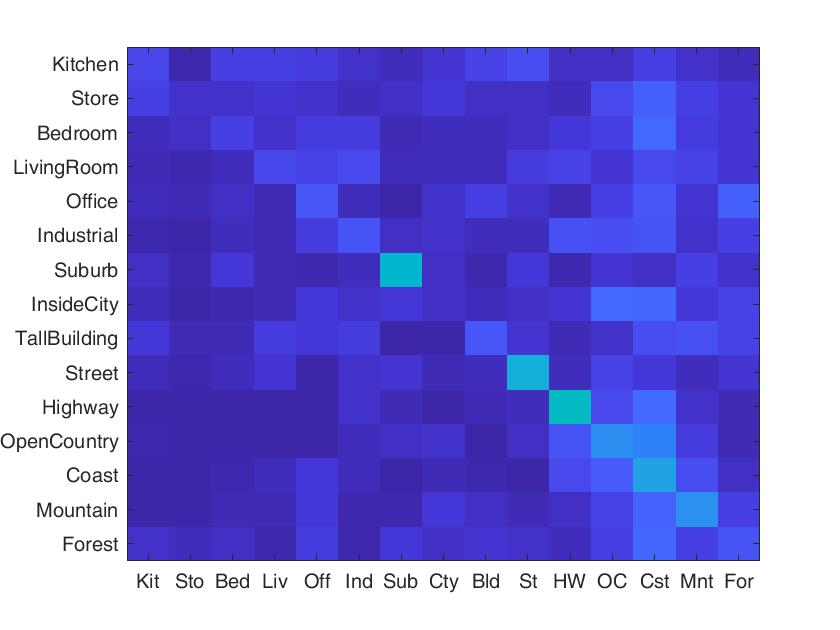
\includegraphics[width=5cm]{ti_nn.jpg}
    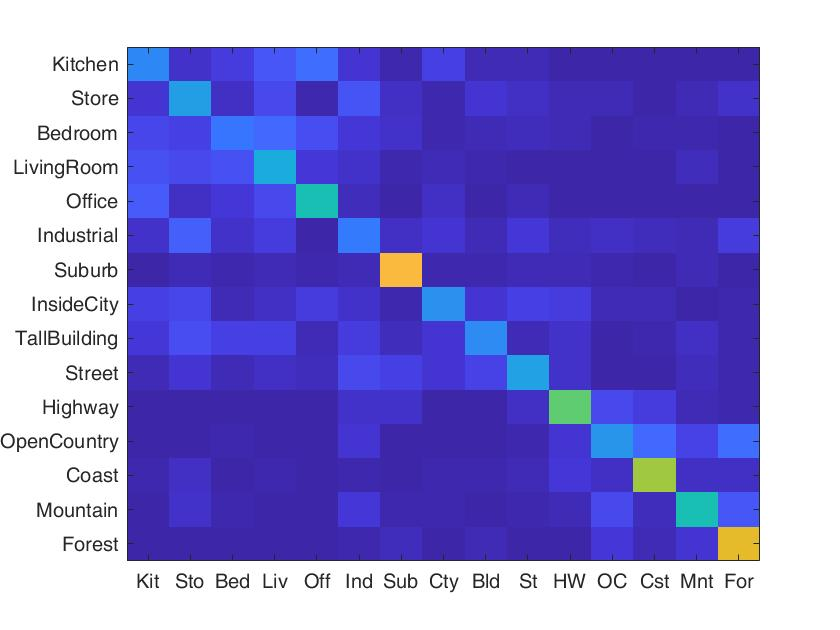
\includegraphics[width=5cm]{bow_nn.jpg}
    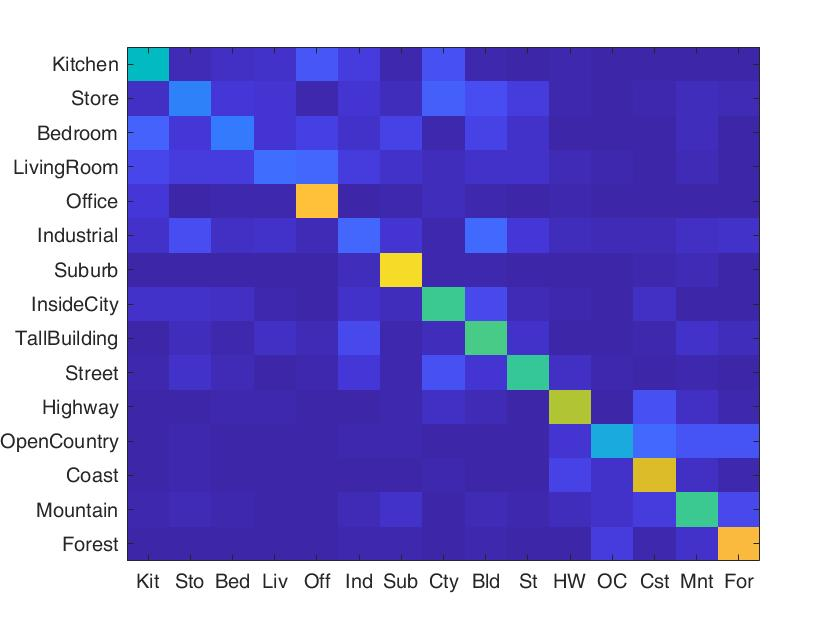
\includegraphics[width=5cm]{bow_svm.jpg}
    \caption{Visualization of my results by methodology \emph{Left-Top:} Random result \emph{Right-Top:} Tiny Image-NN
    \emph{Left-Bottom:} BOW-NN \emph{Right-Bottom:} BOW-SVM}
    \label{fig:result1}
\end{figure}

\end{document}
